%!TEX root = ../document.tex
\chapter{Grundlagen} 
Um die Fragestellungen aus Kapitel \ref{sec:fragestellung} beantworten zu können und eine geeignete Methode zu entwickeln um die Anforderungen zu erfüllen, werden eine Reihe von grundlegenden Verfahren und Begriffen benötigt. 
Der Leser soll hier auf einen Stand gebracht werden, der es ihm ermöglicht die Ausführungen und Ideen nachvollziehen zu können.  
Es werden zunächst Begriffe der sozialen Medien im allgemeinen behandelt um dann den Terminus und die Mechanismen im Twitter-Netzwerk zu erläutern. 
Des weiteren werden besonders die geografischen Aspekte und Möglichkeiten geografischer Angaben in sozialen Medien und insbesondere Twitter erklärt.
Zum Schluss wird die genutzte Datenbasis vorgestellt und erläutert.

\newpage

	\section{Geografische Grundlagen und Begriffe}
	In diesem Kapitel sollen einige geigrafische Grundbegiffe erlätert werden. 
	Die geografischen Begriffe werden in verschiedenen Bereichen unterschiedlich genutzt und teilweise widersprüchlich definiert. 
	Um Missverständnissen vorzubeugen wird hier definiert was unter den einzelnen Begriffen zu verstehen ist.
	Des weiteren folgt eine Reihe von Begriffen die selbst definiert werden um bestimmte Sachverhalte klarer ausdrücken zu können. 

	gesicherte Geoinformationen vs. ungesicherte Geoinformationen+
	unmittelbar geografische Indikatoren
	mittelbar geografische Daten bspsw. Hashtags, Inhaltsanalysen ohne spezielle geografische Hinweise

		\paragraph*{Geodätisches Referenzsystem}
		Ein geodätisches Referenzsystem dient als einheitliche Grundlage zur Angabe einer Position. 
		Geodätische Referenzsysteme sind Koordinatensysteme durch die geografische Koordinaten auf die reale Welt projiziert werden können. 
		In der vorliegenden Arbeit wird das World Geodetic System 1984, kurz wgs84, genutzt.
		Es handelt sich hierbei um ein weit verbreitetes geodätisches Referenzssytem das unter anderem in der Luftfahrt eingsetzt wird.


		\paragraph{Georeferenz}
		Eine Georeferenz (engl. Spatial Reference) wird auch als Raumbezug bezeichnet. 
		Unter dem Begriff der Georeferenz versteht man die Beschreibung der Lage in einem Bezugssystem. 
		Die konkreten Angaben zum Raumbezug und deren Genauigkeit hängt von den Anforderungen ab, die an die Georeferenz gestellt werden. 
		Auch die in \ref{chp:Einleitung} erwähnten Anwednungen stellen unterschiedliche Anforderungen an die Genauigkeit der Georeferenz.
		Die Georeferenz lässt sich weiter unterteilen:
		
			\begin{description}
	 			\item[Direkte Georeferenz (direkter Raumbezug)] Unter direktem Raumbezug versteht man eine Angabe einer konkreten Koordinate bezüglich eines geeigneten, unveränderlichen Bezugssystems. 
	 			Zusätzlich wird eine Genauigkeit angegeben. 
	 			Beispielsweise geographische Koordinaten bezüglich eines geodätischen Referenzsystems. 
	 			\item[indirekter Georeferenz (indirekter Raumbezug) ] Unter indirektem Raumbezug werden alle Angaben verstanden die eine ungenauere Position bestimmen und einem veränderlichen Bezugssystem unterliegen.
	 			Meist beschrieben die Angaben Flächen einer gewissen Ausdehnung.
	 			Beispielsweise Länder, vollständige Adressen, Postleitzahlen oder auch Telefonvorwahlen. 

	 		\end{description}

	 	Aufrgund der einfacheren Verständlichkeit werden die folgenden zwei Begriffe definiert, welche in der restlichen Arbeit verwendet werden.

		\paragraph*{geografische Position}
		Unter geografischer Position wird hier ein konkreter Ort unter Angabe geografischer Koordinaten verstanden.
		Eine geografische Position ist somit eine direkte Georeferenz.

		\paragraph*{geographische Region} 
		Unter einer geografischen Region werden Flächen von geografischer Ausdehnung verstanden. 
		Hierbei kann es sich beispielsweise um Bundesländer oder Länder handeln.
		Somit sind diese Angaben indirekte Georeferenzen

		\paragraph*{Georeferenzierung}
		Unter Georeferenzierung versteht man die Zuordnung einer Georeferenz zu einem Datensatz. 

		


		\subsection{Geoinformationen in Daten sozialer Netzwerke}
	 		\begin{enumerate}
	 			\item \todo{gesicherte und ungesicherte Geoniformationen definieren!} 
	 			\item konkrete Geolocations (bsp. Städte <--> Länder) \cite{Hecht2011}
	 			\item 
	 			\item Lokalisierung von Social-Media Elementen (Videos, User, Nachrichten, Bilder) kleine Übersicht
	 			\item Hinleitung zu Twitter  
	 		\end{enumerate}

		\subsection{Twitter}
			Allgemeine Informationen zu Twitter. 
			\begin{enumerate}
				\item Was ist Twitter -> Tweets/Mechanismen/"'Wie wird Twitter genutzt"''
				\item \todo{Paper raussuchen -> Einfluss von Twitter auf Weltbild/Meinung/ } Einfluss von Twitter auf Weltbild/Meinung/ usw.
				\item Twitter als Nachrichtenmedium (Can Twitter Replace Newswire (Petrovic et. al ))
				\item Anatomie eines Tweets 
					\begin{enumerate}
						\item Welche Informationen sind in einem Tweet enthalten? 
						\item Konzentration auf Daten die Hinweise zur räumlichen Lage geben könnten aber auch allgemein auf die Daten eingehen.
					\end{enumerate}

					\item Definition Twitter-Umfeld
			\end{enumerate} 



	\section{Geographie Daten}


	\section{Data Sample}




\chapter{Stand der Technik} 
	Die Georeferenzierung von Twitter-Kurznachrichten oder Twitter-Nutzern ist ein Feld an dem nach wie vor aktiv geforscht wird.
	Nicht zuletzt trägt auch die große Verfügbarkeit an Twitter-Daten zu dem Umstand bei, dass Twitter in den letzten Jahren Forschungsgegenstand zahlreicher Publikationen war. 
	
	In diesem Abschnitt sollen bestehende Ansätze zur Georeferenzierung im Twitter-Umfeld untersucht werden. 
	Es werden Kriterien zur Einordnung der bestehenden Ansätze erarbeitet und erläutert.   
	Die Arbeiten werden mit Hilfe der Kriterien schematisch eingeordnet um einen Überblick zu erhalten. 
	Zum Schluss wird untersucht ob die Arbeiten die bereits formulierten Anforderungen aus \ref{sec:Anforderungen} erfüllen, und wie sich die vorliegende Arbeit von den bestehenden Ansätzen abgrenzt.    

		\section{Kategorisierung bestehender Ansätze}

		In früheren Arbeiten wurde bereits versucht, eine Einordnung der bestehenden Verfahren vorzunehmen. 
		Es ist interessant die Kategoriesierungsansätze und die verwandten Arbeiten einiger Autoren zu studieren.
		Es lässt sich dadurch die Entwicklung zum Thema Lokalisierung im Twitter-Umfeld beobachten. 
		Einige Kategorisierungsansätze werden im folgenden aufgelistet und erläutert.

		Sowohl in \cite{Hecht2011} als in \cite{Cheng2010} beschränken sich die verwandten Arbeiten nicht auf die Lokalisierung im Twitter-Umfeld, es werden Arbeiten zur Lokalisierung von Web-Inhalten im Allgemeinen aufgelistet. 
		Dies lässt darauf schliessen, dass sich vor den Jahren 2010/2011 nur wenige Arbeiten mit der Lokalisierung im Twitter-Umfeld beschäftigt haben.  
		
		\subsubsection{Kategorisierung über die untersuchte Ressource}
		\cite{Hecht2011} nimmt deshalb eine Kategorisierung anhand der untersuchten Ressource vor. 
		Es wird unterschieden zwischen Forschungen zur "'Lokalisierung von Microblogging-Seiten und deren Inhalten"' und der "'Lokalisierung von Nutzern, welche Inhalte zu Web 2.0 Seiten beisteuern"'. 
		Zusätzlich wird in dieser Arbeit das "'Verhalten der Nutzer im Umgang mit der Veröffentlichung ihres aktuellen Standorts"' und die "'Vorhersage privater Informationen"' betrachtet. Darauf soll hier allerdings nicht weiter eingegangen werden.      

		\subsubsection{Kategorisierung über die verwendete Methode}

		\cite{Cheng2010} klassifiziert die vorgestellten Arbeiten anhand der verwendeteten Methodik. 
		Es wird auf Arbeiten zur Lokalisierung von Webseiten, Web-Logs, Suchanfragen und Web-Nutzern verwiesen. 
		Diese werden in die folgenden drei Kategorien eingeteilt.

		\paragraph*{"'Inhaltsanalyse mit Begriffen in einem geografischen Verzeichnis (Content analysis with terms in a gazetteer)"'}  
		Es wird darunter eine einfache Datenbanksuche verstanden. 
		Es werden einzelne Wörter in einer Datenbank nachgeschlagen um diese einem konkreten geografischen Ort zuweisen zu können.
		Dabei kann sowohl lokal auf eine Geo-Datenbank als auch auf Internet Ressourcen zurückgegriffen werden.  
		In der Regel durchläuft der untersuchte Text eine manuelle oder automatische Vorverarbeitung um potenziell geografische Begriffe, sogenannte Toponyme, herauszufiltern. 

		\paragraph*{"'Inhaltsanalyse mit probabilistischen Sprachmodellen (Content analysis with probabilistic language models)"'}
		Dabei werden Texte oder Textteile einer Twitter-Kurznachricht zu vordefinierten geografischen Regionen wie Ländern oder Städten zugeordnet. 
		Nach einer Vorverarbeitung des Textes erfolgt eine statistische Auswertung, um danach den Text oder einzelne Textteile, wie beispielsweise Wörter, einer geografischen Region zuzuordnen. 
		Eine unbekannter Text kann dann mit Hilfe der zuvor gelernten Zuordnung einer geografischen Region zugeordnet werden.

		\paragraph*{"'Schlussfolgerungen durch soziale Verbindungen (Inference via social relations)"'} es werden soziale Verbindungen, die in Netzwerken abgebildet sind, herangezogen um Rückschlüsse auf den geografischen Ort des untersuchten Inhaltes oder einer Person ziehen zu können.

		Preidhorsky et al. schlagen in \cite{Priedhorsky2013} eine weitere Einteilung anhand der Methodik vor. 
		Allerdings werden hier ausschließlich Arbeiten im Twitter-Umfeld betrachtet. 

		\paragraph*{"'Geocoding"'} Im wesentlichen entspricht dies der "'Inhaltsanalyse mit Begriffen in einem geografischen Verzeichnis"' aus \cite{Cheng2010}. 
		"'Geocoding"' wird als Begriff in vielen Fachrichtungen unterschiedlich definiert, was zu Missverständnissen führen kann. 
		In \cite{bibsmaniaaa:Goldberg2008} wird genauer auf den Begriff des Geocoding und die Poblematik eingegangen und eine Definition  des Begriffs vorgeschlagen.
		Im vorliegenden Kontext ist es präziser und weniger missverständlich die Methodik als "'Inhaltsanalyse mit Begriffen in einem geografischen Verzeichnis"' zu bezeichnen, anstatt den Begriff "'Geocoding"' einzusetzen. 
		
		\paragraph*{"'Geografische Themenmodelle (Geographic Topic Modeling)"'} wird definiert als die Verbindung von "'Themenmodellierung"' und "'Standorterkennung (Location Awareness)"'. 
		Durch klassisches "'Themenmodellierung"' lässt sich aus aus Texten eine Menge von Themen extrahieren. 
		Durch eine Lernphase werden Wörterbücher zu den Themen erstellt.
		Mit Hilfe dieser Themen-Wörterbücher kann später das Thema eines Textes bestimmt werden. \cite{Blei2012} 
		Unter "'Standorterkennung"' wird hier verstanden, dass nicht nur das Thema sondern auch eine bestimmte Region extrahiert werden kann. 
		Dies kann durch geografischen Koordinaten in Twitter-Kurznachrichten realisiert werden. 
		Im Unterschied zur Kategorie "'Inhaltsanalyse mit probabilsitischen Sprachmodellen"' aus \cite{Cheng2010} wird hier jedoch keine vorgegebene geografische Region gefordert. 
		Vielmehr ergeben sich die geografischen Regionen aus den Themenmodellen und den zugehörigen geografischen Koordinaten.
		Es wird damit eine kontinuierliche Region beschrieben, welche nicht zwangsweise durch Stadt-, Staaten- oder Ländergrenzen beschränkt ist.  

		\paragraph*{"'Statistische Klassifizierung (Statistical classifiers)"'} Diese Kategorie entspricht der "'Inhaltsanalyse mit probabilsitischen Sprachmodellen"' wobei in \cite{Cheng2010} nur eine Arbeit in dieser Kategorie betrachtet wird. \cite{Priedhorsky2013} listet mehrere Arbeiten auf, die sich in diese Kategorie einordnen lassen.   

		\paragraph*{"'Informationen aus sozialen Verbindungen (Social Network Information)"'} analog zu "'Schlussfolgerungen durch soziale Verbindungen"' aus \cite{Cheng2010} werden soziale Verbindungen herangezogen um den Standort zu bestimmen. 

		Priedhorsky et al. wählen eine ähnliche Einteilung wie vormals Cheng et al. in 2010, die verwandten Arbeiten stammen allerdings aus dem Twitter-Umfeld. 
		Dabei ist zu bemerken, dass sich die verwendeten Methoden zur Lokalisierung im Twitter-Umfeld nicht wesentlich von denen in anderen Bereichen unterscheiden. 
		Um die Arbeiten im Twitter-Umfeld sinnvoll voneinander abgrenzen zu können muss die Kategorisierung mehr Dimensionen umfassen. 
		Es müssen mehr Kriterien zur Kategorisierung herangezogen werden als die reine Methodik.   

		Mahmud et al. betrachten in \cite{Mahmud2012} hauptsächlich Arbeiten im Twitter-Umfeld. 
		Diese werden in die folgenden Kategorien unterteilt. 

		\begin{enumerate}
			\item  "'Inhaltsbasierte Standortschätzung von Tweets (Content-based Location Estimation from Tweets)"'
			\item "'Inhaltsbasierte Standortextrahierung von Tweets (Conetnt-based Location Extraction from Tweets"'
			\item "'Standortschätzung ohne den Tweet Inhalt zu nutzen (Location Estimation without using Tweets Content)"'
		\end{enumerate}

		\paragraph*{"'Inhaltsbasierte Standort-Schätzung von Tweets (Content-based Location Estimation from Tweets)"'} hier wird die geografische Position durch eine Inhaltsanalyse der Twitter-Kurznachricht geschätzt. 
		Die Schätzung erfolgt dabei durch probabilistische Modelle.
		Diese Kategorie vereint damit "'Geografische Themenmodelle"', "'Statistische Klassifizierung"' aus \cite{Priedhorsky2013} mit "'Inhaltsanalyse mit probabilsitischen Sprachmodellen"' aus \cite{Cheng2010} und ist damit als genereller anzusehen, als die vorgenannten Kategorien. 

		\paragraph*{"'Inhaltsbasierte Standort-Extrahierung von Tweets (Conetnt-based Location Extraction from Tweets"'} die verwandten Arbeiten in dieser Kategorie versuchen direkte Hinweise auf einen geografischen Ort aus einer Twitter-Kurznachricht zu extrahieren. 
		Diese Kategorie ähnelt dem "'Geocoding"' beziehungsweise der "'Inhaltsanalyse mit Begriffen in einem geografischen Verzeichnis"'. 

		\paragraph*{"'Standortschätzung ohne den Tweet Inhalt zu nutzen (Location Estimation without using Tweets Content)"'} hierunter versteht der Autor alle Informationen die nicht unmittelbar in der Twitter-Kurznachricht enthalten sind. Dazu zählen Informationen aus dem Nutzerprofil oder Informationen über die sozialen Verbindungen des Nutzers.


		\cite{Mahmud2012} nutzt ebenfalls die Methodik um die Arbeiten zu kategorisieren. 
		Allerdings wird hier eine generellere Einteilung vorgenommen. 
		So wird unterteilt, ob der Standort geschätzt oder extrahiert wurde.  
		Mahmud et al. bringen aber auch eine weitere Dimension ein. 
		Es wird hier zusätzlich unterschieden ob das angewendete Verfahren den Tweet-Inhalt nutzt oder andere Informationen. 

		Dies ist sinnvoll, denn die genannten Methoden lassen sich sowohl auf den Tweet-Inhalt als auch auf andere Informationen, beispielsweise aus dem Nutzerprofil, anwenden.     



		
		Frühere Arbeiten verweisen auf ein weiteres Spektrum an Arbeiten aus anderen Bereichen, wie Lokalisierung von Flickr Bildern oder Web-Log Einträgen.
		Arbeiten zur Lokalisierung im Twitter-Umfeld werden hier seltener erwähnt. 
		In späteren Arbeiten, wie in \cite{Priedhorsky2013}, wird hingegen fast ausschließlich auf Arbeiten aus dem Twitter-Umfeld verwiesen. 
		Dies spiegelt die steigende Anzahl der Arbeiten zur Lokalisierung im Twitter-Umfeld wieder.
		Betrachtet man die Ausarbeitungen zur Lokalisierung im Twitter-Umfeld genauer, wird allerdings schnell klar, dass die Kategorisierung der Arbeiten anhand der verwendeten Methodik, dem Umfang nicht mehr gerecht wird. 

		
		
		Bei genauerer Betrachtung der Arbeiten stellt man allerdings fest, dass diese Klassifizierungen dem Umfang der Arbeiten nicht gerecht wird. 
		\cite{Hecht2011} verweist auf ähnliche Ansätze mit einem anderen Untersuchungsgegenstand.
		\cite{Cheng2010} kategorisiert die Arbeiten anhand der Methodik, und verweist ebenso auf andere Untersuchungsgegenstände. 
		\cite{Priedhorsky2013} verweist ausschliesslich auf Arbeiten im Twitter-Umfeld und kategorisiert diese anhand der verwendeten Methodik. 
		Die Methodeneinteilung ist aufgrund der Begriffswahl missverständlich und kann somit zu Problemen führen. 

		\subsection{ttt<sss}


		In \cite{Schulz2013} werden die folgenden Dimensionen zur Abgrenzung herangezogen.




		Allerdings lassen sich noch andere Dimensionen zur Klassifizierung der Arbeiten heranziehen. 
		Wird besipielsweise der Text einer Twitter-Kurznachricht durch eine einfache Geokodierung untersucht wird dies andere Ergebnisse liefern als eine Untersuchung auf Basis eines geografischen Themenmodells.  
		





		\cite{Hecht2011} nutzen diese Methode um eine Ground-Truth zu bestimmen indem das Userlocation-Feld in Wikipedia nachschlagen wird. Wikipedia bietet zu vielen Artikeln eine grografische Position in Form von Längen- und Breitengrad an, diese werden dann der untersuchten Twitter-Kurznachricht zugeordnet. 
		\cite{Hale2012} nutzen die Yahoo und die Google Geocoding Api um das Userlocation-Feld eingehender zu untersuchen.  
		

		
		Eine weitere zu betrachtende Dimension stellt daher der konkrete Untersuchungsgegenstand in Form des Indikators dar.


		Betrachtet man die Gesamtheit an arbeiten im Bereich der Lokalisierung im Twitter Netzwerk drängen sich noch mehr Dimensionen zur Klassifizeirung der arbeiten auf.

		

		\begin{enumerate}
		 	\item Räumliche Indikatoren
		 	\item Techniken
		 	\item Fokus der Lokalisierung
		 \end{enumerate} 	









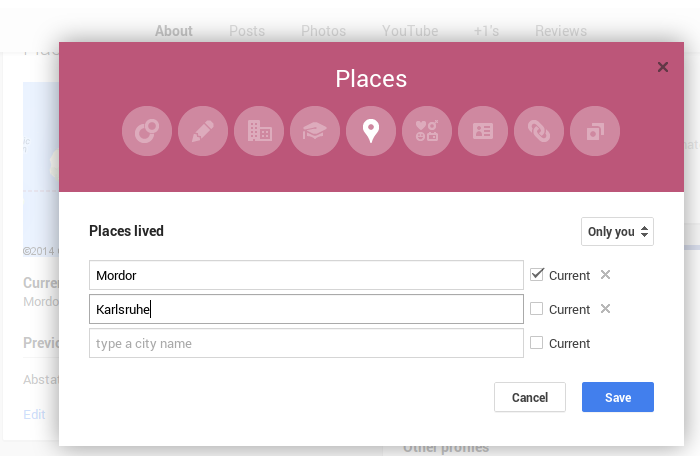
\includegraphics[scale=0.7]{gPlusPlaces.png}

		\begin{enumerate}
			\item Naiver Ansatz -> Geocoding mit Google Maps API V3, nur Indikatoren die geografische Namen enthalten. 
					Prinzipiell einfache Datenbankabfrage mit ein wenig semantik. 
					Keine Jargon Namen wie Big Apple etc.
				\begin{enumerate}
					\item Funktion der GMaps Api V3
					\item Einschränkungen der GMaps Api V3
					\item zurückgelieferte Daten der GMaps Api V3
					\item Kurze Beschreibung wie ich die API genutzt habe
				\end{enumerate}
			\item aktuelle Ansätze
				\begin{enumerate}
					\item{\todo{Ist das grundsätzliche Verfahren, analysieren Inhalt/Indikatoren -> Zuordnen auf geografische Angaben und danach Clustern tatsächlich immer gleich bei allen Arbeiten? kontinuierlich vs diskrete geografische Daten} 
					allgemeiner Ansatz : Geotagged Tweets analysieren (Inhalt/andere Indikatoren usw. ), zuordnen zu geografischen \"Bereichen\" und daraus lernen.}
					\item Verfahren mit Inhaltsanalysen
					\item Verfahren mit Indikatoren einzelne oder mehrere
					\item Welche Verfahren kommen beim mapping auf \todo{geografische Entität definieren} geografische Entitäten zum Einsatz
				\end{enumerate}
		\end{enumerate}

		\subsection{Probleme früherer Ansätze}
			\begin{enumerate}
				\item{Genutzte API's und Indikatoren nur in bestimmten Sprachen verfügbar}
				\item{keine Schätzung für Genauigkeit auf verschiedenen geografischen Hierarchieebenen verfügbar}  
			\end{enumerate}

	
	
	

	
